\chapter{Validación de la aplicación por usuarios reales}
\label{cap:validacion}

En esta sección se aborda la validación de la aplicación mediante pruebas realizadas con usuarios reales. Este proceso constituye una etapa fundamental en el desarrollo de software, ya que permite evaluar la usabilidad, funcionalidad y experiencia general del sistema en un entorno práctico y representativo.

El propósito principal de estas pruebas es garantizar que la aplicación cumpla con los estándares de calidad esperados y satisfaga las necesidades de los usuarios finales. A través de la interacción directa con el sistema, los usuarios pueden proporcionar información valiosa que ayuda a identificar posibles problemas, como errores en el diseño, dificultades en la navegación, o características que no cumplen con las expectativas. Asimismo, estas pruebas permiten confirmar los aspectos positivos del diseño que contribuyen a una experiencia de usuario satisfactoria.

La validación con usuarios reales no solo se centra en detectar áreas de mejora, sino también en recopilar datos cuantitativos y cualitativos. Además, este tipo de pruebas permite evaluar la satisfacción del usuario mediante herramientas como cuestionarios para medir el sistema. Los resultados obtenidos a partir de estas evaluaciones son esenciales para tomar decisiones informadas sobre posibles ajustes y mejoras en el diseño.

En resumen, el objetivo de este proceso de validación es doble: por un lado, identificar y corregir problemas de usabilidad o funcionalidad que puedan afectar negativamente la experiencia del usuario; y por otro, confirmar que el sistema desarrollado es intuitivo, eficiente y agradable de utilizar en escenarios reales. Este enfoque centrado en el usuario asegura que la aplicación no solo cumpla con los requisitos técnicos, sino que también ofrezca una experiencia de alta calidad que satisfaga las expectativas de quienes la utilizan.



\section{Preparacion de la prueba}

Para llevar a cabo la validación de la aplicación, se comenzó con la preparación del entorno de prueba, asegurando que los usuarios pudieran interactuar con la aplicación de manera eficiente y sin complicaciones técnicas. Este proceso inicial es crucial para garantizar que las pruebas se desarrollen en condiciones óptimas y que los resultados obtenidos sean representativos y fiables.

En primer lugar, se realizó una investigación sobre las diferentes opciones disponibles para proporcionar acceso a la aplicación a los usuarios. Se evaluaron diversas alternativas, como la distribución mediante archivos APK, o la implementación de servicios de despliegue en la nube. Cada opción fue analizada en términos de facilidad de uso, accesibilidad, y compatibilidad con los dispositivos de los usuarios.

Tras considerar las ventajas y desventajas de cada alternativa, se decidió utilizar un servicio proporcionado por Firestore. Este servicio ofrece una solución eficiente y práctica para desplegar aplicaciones desarrolladas en Flutter. Mediante el uso de Firestore, se pudo compilar la aplicación directamente desde el código fuente y desplegarla en un servidor accesible a través de Internet. Este proceso genera un enlace único que permite a los usuarios acceder a la aplicación de manera sencilla, sin necesidad de descargar ni instalar archivos adicionales.

El uso de Firebase no solo facilitó el acceso a la aplicación, sino que también proporcionó un entorno seguro y confiable para las pruebas. Además, esta solución permitió realizar actualizaciones rápidas en caso de que se detectaran problemas durante las pruebas, asegurando que los usuarios siempre tuvieran acceso a la versión más reciente de la aplicación.

Una vez que se garantizó el acceso a la aplicación, lo siguiente fue elegir que tipo de cuestionarios se iban a utilizar para evaluar la experiencia de los usuarios. Los dos cuestionarios más utilizados para evualar 
la usabilidad de una aplicación y que nos prorcionan una puntuación cuantiativa son: 

\begin{enumerate}
    \item \textbf{System Usability Scale (SUS)}: Su objetivo es proporcionar un test fácil de comprender, fácil de puntuar. Permite establacer comparaciones de unas soluciones con otras. Consta de 10 preguntas con una escala del 1 al 5.
    \item \textbf{Software Usability Measurement Inventory (SUMI)}: Este cuestionario es más extenso y permtie evaluar nuevos productos, efectuar comparaciones con versiones previas y establecer objetivos para desarrollos futuros. El cuestionario consta de 50 preguntas que hay que responder con \textit{de acuerdo, no lo sé o en desacuerdo}.
\end{enumerate}


Se decidió utilizar el cuestionario SUS, ya que es más sencillo y rápido de completar, lo que facilita la participación de los usuarios. Además, su formato permite obtener una puntuación cuantitativa que puede ser utilizada para comparar la usabilidad de la app. 

Las preguntas que forman dicho cuestionario son las siguientes:
\begin{enumerate}
    \item Creo que me gustaría utilizar este aplicación con frecuencia.
    \item Encontré la aplicación innecesariamente compleja.
    \item Pensé que la aplicación es fácil de usar.
    \item Creo que necesitaría la ayuda de una persona con conocimientos técnicos para poder usar esta aplicación.
    \item Encontré que las distintas funciones de la aplicación estaban bien integradas.
    \item Pensé que había demasiada inconsistencia en esta aplicación.
    \item Imaginé que la mayoría de las personas aprenderían a usar esta aplicación muy rápidamente.
    \item Encontré la aplicación muy incómoda de usar.
    \item Me sentí muy confiado al usar la aplicación.
    \item Necesité aprender muchas cosas antes de poder utilizar esta aplicación.
\end{enumerate}

Con estas preguntas se creó un formulario en Google Forms, para poder enviárselo a los usuarios posteriormente. 

A pesar de que el cuestionario SUS es muy útil para obtener una puntuación cuantitativa, no proporciona una información 
específica sobre los aspectos que los usuarios consideran positivos o negativos de la aplicación. Por lo tanto, se decidió complementar con otro cuestionario con preguntas más abiertas y específicas realizadas por mi.
Las preguntas que se realizaron fueron las siguientes: 

\begin{enumerate}
    \item Me ha resultado fácil crear una lista de la compra.
    \item Añadir productos a una lista es intuitivo.
    \item El proceso para añadir un gasto es sencillo.
    \item Entiendo bien cómo se reparten los gastos entre los miembros del hogar.
    \item Encuentro fácilmente las tareas semanales o puntuales asignadas.
    \item Crear una nueva tarea es rápido y claro.
    \item La visualización de la planificación semanal me parece útil.
    \item Navegar entre secciones como listas, tareas y gastos es fácil.
    \item El diseño y colores de la aplicación me parecen agradables.
    \item La aplicación funciona de forma fluida y rápida.
    \item La manera de ver los datos del perfil es intuitiva.   
    \item La pantalla principal, sirve para hacerte una idea general de todo lo que ofrece la app.
    \item ¿Qué funcionalidad de la app te ha parecido más útil? ¿Por qué?.
    \item ¿Hubo alguna funcionalidad que te costó entender o usar?.
    \item ¿Qué mejorarías o cambiarías en la aplicación?.
    \item ¿Añadirías alguna funcionalidad nueva? ¿Cuál?.
    \item ¿Tuviste algún problema o error técnico? Si es así, descríbelo.


\end{enumerate}

De la pregunta 1 a la 12 se les pidió a los usuarios que puntuaran de 1 a 5 siendo 1 muy en desacuerdo y 5 muy de acuerdo. Mientras que 
las preguntas de la 13 a la 17 eran abiertas, para que los usuarios pudieran expresar su opinión de forma más detallada.

Una vez que se creó este último cuestionario, lo único que quedaba era reclutar a los usuarios que iban a participar en la prueba. 
Encontrar a usuarios representativos era fácil ya que la aplicación está diseñada para ser utilizada por estudiantes que comparten piso y 
por edad y estilo de vida, la mayoría de mis amigos y compañeros de clase encajaban en este perfil.


\section{Realización de la prueba}




\begin{figure}[h]
    \centering
    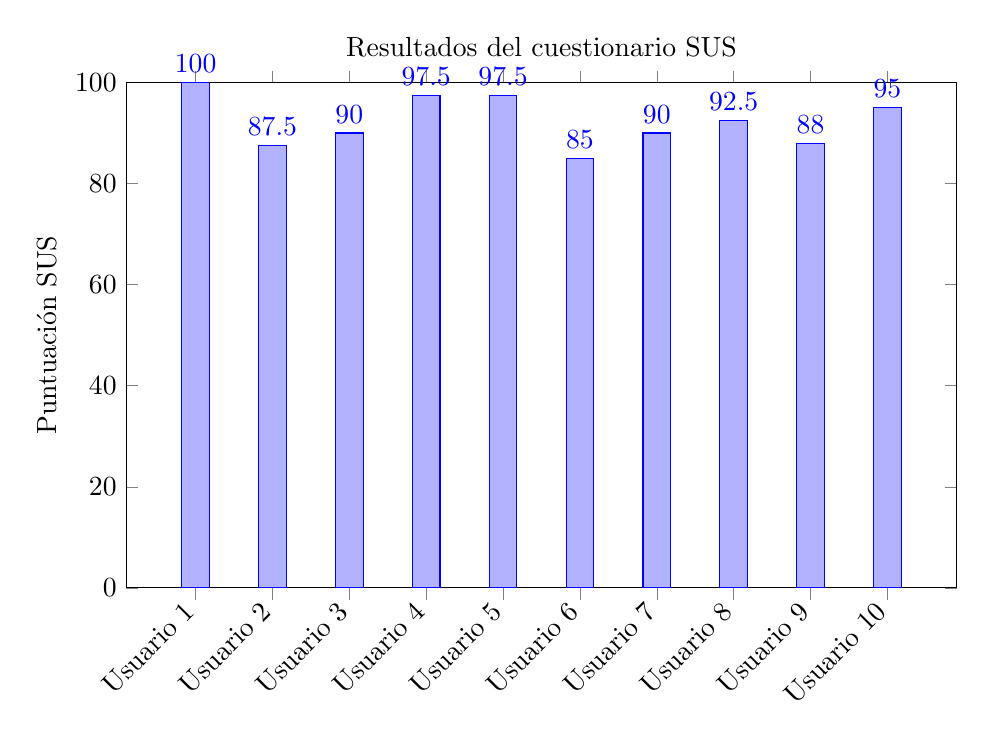
\begin{tikzpicture}
    \begin{axis}[
        ybar,
        bar width=10pt,
        ymin=0, ymax=100,
        ylabel={Puntuación SUS},
        symbolic x coords={Usuario 1, Usuario 2, Usuario 3, Usuario 4, Usuario 5, Usuario 6, Usuario 7, Usuario 8, Usuario 9, Usuario 10},
        xtick=data,
        nodes near coords,
        nodes near coords align={vertical},
        width=\linewidth,
        height=8cm,
        title={Resultados del cuestionario SUS},
        x tick label style={rotate=45, anchor=east}
    ]
    \addplot coordinates {
        (Usuario 1, 100)
        (Usuario 2, 87.5)
        (Usuario 3, 90)
        (Usuario 4, 97.5)
        (Usuario 5, 97.5)
        (Usuario 6, 85)
        (Usuario 7, 90)
        (Usuario 8, 92.5)
        (Usuario 9, 88)
        (Usuario 10, 95)
    };
    \end{axis}
    \end{tikzpicture}
    \caption{Puntuaciones individuales SUS}
\end{figure}

